\documentclass[a4paper,11pt,titlepage]{article}
\usepackage{graphicx}
\author{Abrie Greeff\\B.Sc Hons (Computer Science)\\Department of Computer Science\\University of Stellenbosch}
\title{Advanced Algorithms: Homework 1}
\begin{document}
\maketitle
\tableofcontents
\section{R-5.3}
Skedulering van $T={(1,2),(1,3),(1,4),(2,5),(3,7),(4,9),(5,6),(6,8),(7,9)}$
\begin{figure}[htbp]
   \centering
   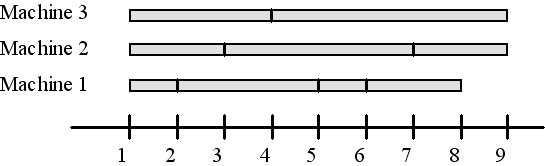
\includegraphics[width=10cm]{sched.png}
   \caption{Skedulering van T}
   \label{Figure:figex}
\end{figure}

\section{R-5.4}
\subsection{(a)}
$T(n) = 2T(n/2) + logn\\
a = 2, b = 2\\
n^{log_22} = n$\\
Case 2 met k = 1\\
$T(n)$ is $O(nlog^2n)$\\
\subsection{(b)}
$T(n) = 8T(n/2) + n^2\\
a = 8, b = 2\\
n^{log_28} = n^3$\\
Case 1 met $\epsilon$ = 1\\
$T(n)$ is $\theta(n^3)$\\
\subsection{(c)}
$T(n) = 16T(n/2) + (nlogn)^4\\
a = 16, b = 2\\
n^{log_216} = n^4$\\
Case 2 met k = 4\\
$T(n)$ is $\theta(n^4log^5n)$\\
\subsection{(d)}
$T(n) = 7T(n/3) + n\\
a = 7, b = 3\\
n^{log_37} = n^{1.77124}$\\
Case 1 met $\epsilon = 0.77124$\\
$T(n)$ is $\theta(n^{1.77124})$\\
\subsection{(e)}
$T(n) = 9T(n/3) + n^3logn\\
a = 9, b = 3\\
n^{log_39} = n^3$\\
Case 2 met k = 1\\
$T(n)$ is $\theta(n^3log^2n)$\\

\section{R-5.6}
Z = XY\\\\
\begin{math}
X = \left[
\begin{array}{clrr}
3 & 2\\
4 & 8
\end{array}
\right]
\end{math}
\begin{math}
Y = \left[
\begin{array}{clrr}
1 & 5\\
9 & 6
\end{array}
\right]\\\\
S_1 = 3(5 - 6) = -3\\
S_2 = (3 + 2)6 = 30\\
S_3 = (4 + 8) = 12\\
S_4 = 8(9 - 1) = 64\\
S_5 = (3 + 8)(1 + 6) = 77\\
S_6 = (2 - 8)(9 + 6) = -90\\
S_7 = (3 - 4)(1 + 5) = -6\\
\\
I = S_5 + S_6 + S_4 - S_2 = 21\\
J = S_1 + S_2 = 27\\
K = S_3 + S_4 = 76\\
L = S_1 - S_7 - S_3 + S_5 = 68\\
\\
Z = \left[
\begin{array}{clrr}
21 & 27\\
76 & 68
\end{array}
\right]\\
\end{math}
\section{R-5.7}
\begin{math}
(a + bi)(c + di) = e + fi\\
(ac - bd) + (ad+bc)i = e + fi\\
\\
\begin{array}{clrr}
ac - bd = e & ad + bd = f\\
ac - b(c+d) + bc = e & ad + b(c+d) - bd = f\\
c(a+b) - b(c+d) = e & b(c+d) + d(a-b) = f
\end{array}
\end{math}
\\

Dus om $e + fi$ in slegs drie vermenigvuldig operasies te bereken moet die volgende drie uitgevoer word:\\
\\
\begin{math}
c(a+b)\\
d(a-b)\\
b(c+d)
\end{math}
\section{R-5.9}
Gegee die matrikse:
A is 10x5\\
B is 5x2\\
C is 2x20\\
D is 20x12\\
E is 12x4\\
F is 4x60

As die greedy method (minste vermenigvuldig operasies) gebruik word om $ABCDEF$ op te los dan word die volgende gekry:
\\
\begin{math}
A \cdot B\\
(A \cdot B)\cdot C\\
((A \cdot B)\cdot C)\cdot (D \cdot E)\\
(((A \cdot B)\cdot C)\cdot (D \cdot E)) \cdot F\\
100 + 400 + 960 + 800 + 2400 = 4660\\
\end{math}
\\
Dit sal dus 4660 vermenigvuldig operasies vat om te bereken.

\section{P-5.2}

\subsection{Fractional Knapsack}
Om uit te voer tik in \emph{java FraqKnapsack}.
\subsection{0-1 Knapsack}
Om uit te voer tik in \emph{java Knapsack}.
\subsection{Bruteforce 0-1 Knapsack}
Om uit te voer tik in \emph{java bruteKnapSack}.
\end{document}
